\chapter{Methodology}
\label{chap:2}
\ChapterPageStuff{2}

\section{Preamble}\label{sec:ch2_preamble}
 The literature in \Cref{chap:1} is used for the method to create a logging mechanism that can capture user-based activity logs to improve software maintenance by analysing the obtained logs. The Web-based application system on this logging mechanism will be implemented on is an energy management system for the mining industry.\par In \Cref{fig:ch2_webSystemBasic} is the basic design of the Web application the users interact with where each mine group has different toolboxes linked to it and each toolbox has different dashboards linked to them which the users can access and interact with. The activities of each of these dashboards and how the user navigates through them are necessary for the system utilisation analysis.

\begin{figure}[!htb] % An h :here, t: top, b: bottom.
	\centering % cent the figure
	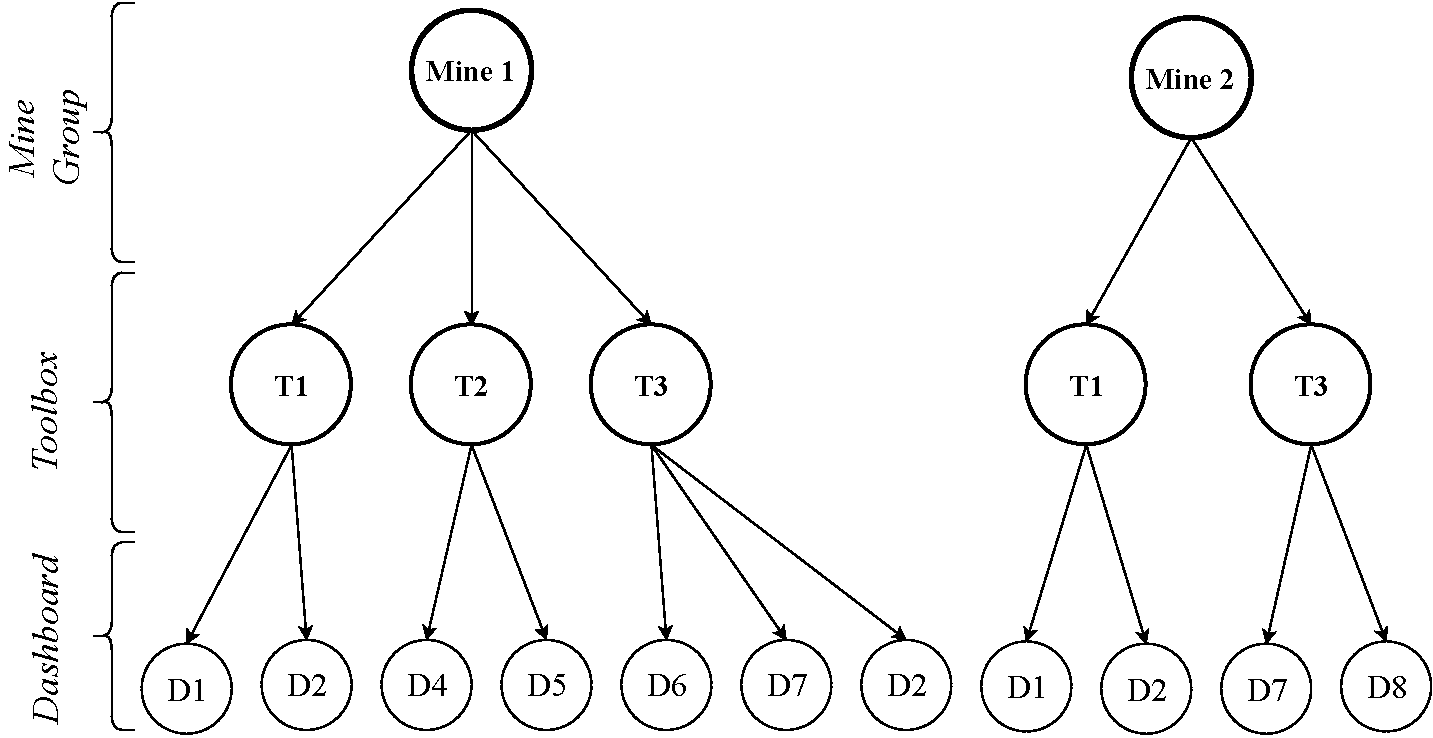
\includegraphics[width=0.85\textwidth]{Chapter2/SystemA_Dashboard/SystemA_Dashboard.pdf}
	\caption[Basic design of an energy management system]
	{\textit{Basic design of an energy management system}}\label{fig:ch2_webSystemBasic}
\end{figure}

In \Cref{Ch2:LoggingMechanism} the methodology to create a logging mechanism to capture user-generated events is discussed for web-based applications. The different functional requirements and interfaces are discussed in this section \cite{Anish2015}.\par In \Cref{ch2:sec_system_utilisation_analysis} the methodology is discussed to analyse these obtained logs to improve software maintenance by using various tools visualisation tools or creating them based on the log attributes that are available.

\section{Logging mechanism}\label{Ch2:LoggingMechanism} The logging mechanism will need to meet the requirements discussed in \Cref{sec:ch1_eventLogging} to capture the required logs to apply system utilisation analysis on it. \Cref{fig:ch2_systemDesign} is the design for the logging mechanism to capture the user's activities. In this figure, the logging mechanism is split up into two functional requirements parts (F/R) which consist of the client and server functional requirements.\par Each functional requirement has an interface requirement that transfers the data from one interface to another interface. These interfaces are labelled as I/F in \Cref{fig:ch2_systemDesign}. The \Cref{fig:ch2_systemDesign} is the client interface (\phase{fr:client}) and the server interface (\phase{fr:server}) that forms the entire logging mechanism to capture the user-based activity logs.

\begin{figure}[!htb] % An h :here, t: top, b: bottom.
	\centering % cent the figure
	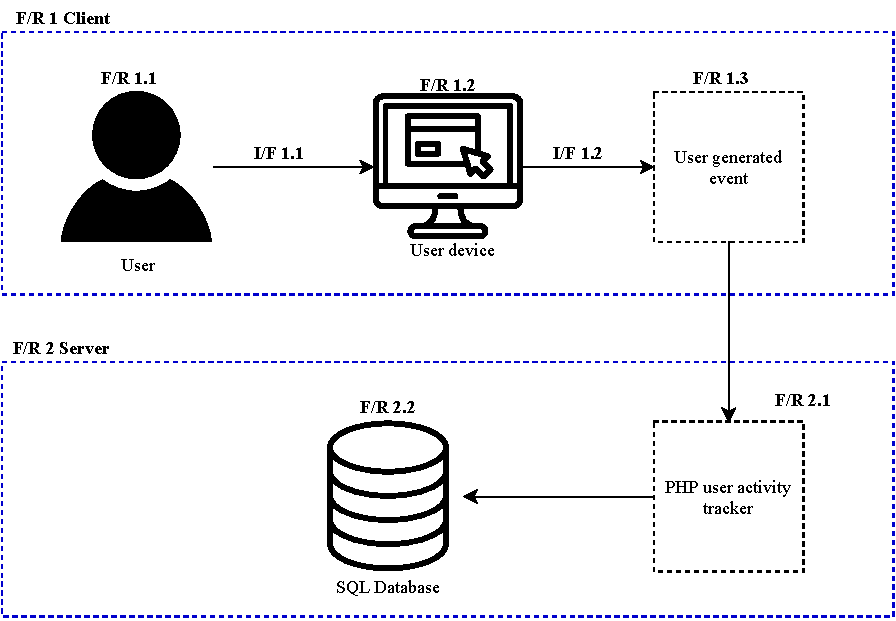
\includegraphics[width=0.9\textwidth]{Chapter2/SystemA_Architecture_Diagram/SystemA_Architecture_Diagram.pdf}
	\caption[Logging mechanism architecture design]
	{\textit{Logging mechanism architecture design}}\label{fig:ch2_systemDesign}
\end{figure}

\subsubsection{Clients functional requirements}
The client's functional requirements (F/R 1) are where the user-based activity is triggered. In \Cref{fig:ch2_systemDesign} the client interface consists of three main functional requirements. These interfaces in \Cref{tbl:ch2_clientFunctionalRequirements} parses the input from the user to create a basic user-based action that can be parsed and captured and parsed by the logging point to create a user-based log that is parsed onto the server for further processing.

\setcounter{phase}{1}
\begin{table}[!htb]
	\centering
	\caption[Client functional requirements]
	{\textit{Client functional requirements (F/R 1)}}
	\label{tbl:ch2_clientFunctionalRequirements}
	\begin{tabularx}{\textwidth}{|l|l|X|}
		\hline \textbf{Requirement ID} & \textbf{Name} & \textbf{Description} \\
		\hline \subphase{fr:clientUser} & User & The user serves as the primary initiator of the user-based activity events.\\
		\hline \subphase{fr:clientUserDevice} & User's device & The device that the user uses to access the website from where the user-based activity events are generated.\\
		\hline \subphase{fr:clientUserEvents} & User-generated events & These are the captured user-based activity events that have been identified by the logging point and will be sent to the server.\\
		\hline
	\end{tabularx}
\end{table}

\subsubsection{Server's functional requirements}\label{sec:ch2_serverFunctionalRequirements}
The server functional requirements in \Cref{tbl:ch2_serverInterfaceRequirements} for \Cref{fig:ch2_systemDesign} is the rest of the logging mechanism. At this stage, the obtained user-generated event of \Cref{fig:ch2_user_based_actvity_classification} will be attempted to be completed into a user-based activity log and stored in a database by the logging point. \par 

\stepcounter{phase}
\begin{table}[!htb]
	\centering
	\caption[Server functional requirements]
	{\textit{Server functional requirements (F/R 2)}}
	\label{tbl:ch2_serverInterfaceRequirements}
	\begin{tabularx}{\textwidth}{|l|l|X|}
		\hline \textbf{Requirement ID} & \textbf{Name} & \textbf{Description} \\
		\hline \subphase{fr:serverActivityLogger} & User activity logger & The logging points are used to capture and create the user-based event log that will be stored in a database.\\
		\hline \subphase{fr:serverDatabase} & Database & The event log is stored in a database until it is needed for further analysis.\\
		\hline
	\end{tabularx}
\end{table}

\subsection{Requirements for a user-based activity log}\label{sec:ch2_requirementsOfUAT}
The user is the initiator of the logging mechanism. Each action or event they trigger by interacting with the user interface on their device (F/R 1.2) can be a potential user-generated event. In
\Cref{tbl:ch2_requirementsForUserActivtyEvent} is the sub-requirements for the user (\ref{fr:clientUser}) which the event log should fulfil to be classified as an user-based activity log.

\setcounter{phase}{1}
\setcounter{subphase}{1}
\begin{table}[!htb]
	\centering
	\caption[Requirements for an event to be a user-based activity]
	{\textit{Requirements for an event to be a user-based activity}}
	\label{tbl:ch2_requirementsForUserActivtyEvent}
	\begin{tabularx}{\textwidth}{|l|X|}
		\hline \textbf{Requirement ID} & \textbf{Description}\\
		\hline \subsubphase{fr:requirementsUserBased1} & The event has to be triggered by the user interacting with the user interface using their device and not any other events that the system will self-initiate. The user needs to have interacted with the UI directly. This can also be validated by tracking if the user did interact with the UI from the HTML element ids. \\
		\hline \subsubphase{fr:requirementsUserBased2} & The event must consist of different cases ($ca~ \epsilon~CA$ the cases consists of events) which are noteworthy to make the event log identifiable \cite{Slaninova2014}. \\
		\hline \subsubphase{fr:requirementsUserBased3} & For certain types of event logs for \ref{fr:requirementsUserBased2}, the user-generated event should have an origin from which the event took place. \\
		\hline \subsubphase{fr:requirementsUserBased4} & The event log should consist of attributes that expand the identity of the user-based activity. \\
		\hline \subsubphase{fr:requirementsUserBased5} & The event must have the user as the initiator or input for the user-based activity. This will exclude all events triggered by the system as the user did not directly start the event. \\
		\hline \subsubphase{fr:requirementsUserBased6} & Only use the first \textit{HTTP requests}\footnote{A \textbf{HTTP request} is made by a client, to a named host, which is located on a server. The request aims to access a resource on the server. \cite{IBM2021}.} that is sent to the server. \\ 
		\hline
	\end{tabularx}
\end{table}

Every interaction the user has with the user interface of the device to the software system can be seen as an event triggered by the user. Most of these events won't have a meaningful impact as they won't fulfil \ref{fr:requirementsUserBased2} and \ref{fr:requirementsUserBased4} in \Cref{tbl:ch2_requirementsForUserActivtyEvent}.\par For the user activity event to meet the requirement of \ref{fr:requirementsUserBased2} it has to have defined cases that describe the activity type of each event. These activity types form the basic criteria for which events can be parsed which significantly reduces the number of logs that will be obtained. This will ensure that the event logging process will produce quality user-based logs as discussed in \Cref{sec:ch1_loggingQuality}:

\begin{itemize}
	\item A basic structural complexity to simplify log parsing and development of the logging points in the system,
	\item Keep the logging consistent by not deviating from the defined cases, and
	\item Ensure that the event log's other attributes are complete and available to increase the accuracy and trustworthiness of the event logging when further system utilisation analysis needs to be done. 
\end{itemize}

\subsection{User activity types}\label{sec:ch2_userActivityTypes}
The user-activity logs will be split into three main event types as in \Cref{tbl:ch2_userActivityTypes}. The general user activity event type (\ref{fr:uatType3}) will the be most common user activity event and be split up into different user activity events. This is determined by the need of what utilisation stage requires to analyse specific user activity events. 

\stepcounter{subphase}
\begin{table}[!htb]
	\centering
	\caption[User activity types]
	{\textit{User activity types}}
	\label{tbl:ch2_userActivityTypes}
	\begin{tabularx}{\textwidth}{|l|l|X|}
		\hline \textbf{Requirement ID} & \textbf{Activity Type} & \textbf{Description} \\
		\hline \subsubphase{fr:uatType1} & Web page accessed & The user may navigate through different web pages in a session.\\
		\hline \subsubphase{fr:uatType2} & Session changes & This is any user activities excluding \ref{fr:uatType1} that modifies the user's session:
		\begin{itemize}
			\item Logging into a Web application. Both Successful and failed attempted logins. This user-based activity may cause the log attributes that identify the user will be a \texttt{NULL} value as the user's session has not started yet to verify their identity,
			\item Ending their session through by logging out or declining to extend their session when it is about to expire,
			\item Modifying any session or other relevant variables that can be used in the utilisation analysis
		\end{itemize}\\
		\hline \subsubphase{fr:uatType3} & General activity & Any events excluding the first two user-based activity types that the user initiates when they interact with the web page. Most of the user activity logs will
		have this event type.\\ 
		\hline
	\end{tabularx}
\end{table}

These user activity types can be further expanded in general activity (\ref{fr:uatType3}) for analysis purposes. The general activity types will be different for each system based on what the system enables the user to do or what is needed for further system utilisation analysis such as determining if the action the user triggered was to generate a report that they downloaded.

\clearpage

\subsection{Logging points}\label{sec:ch2_loggingPoints}
In \Cref{sec:ch1_loggignPoints} the logging points should be strategically placed in the software system to capture the log attributes for the user-based activity log. To meet the requirements of \Cref{tbl:ch2_requirementsForUserActivtyEvent} for a user-based activity the logging points should adhere to the logging points functional requirements of \Cref{tbl:ch2_loggingPointRequirement}.

\stepcounter{subphase}
\begin{table}[!htb]
	\centering
	\caption[Logging points requirements]
	{\textit{Logging points requirements}}
	\label{tbl:ch2_loggingPointRequirement}
	\begin{tabularx}{\textwidth}{|l|X|}
		\hline \textbf{Requirement ID} & \textbf{Description} \\
		\hline \subsubphase{fr:lp1} & The logging point should be placed where the user's interaction with the software system will send a \textit{request} back to the server.\\
		\hline \subsubphase{fr:lp2} & Each logging point should consistently capture the user-based activity as the activity is happening. \\
		\hline \subsubphase{fr:lp3} & Logging points should be globally complete to capture the user-based activities in the giving software system without too much modification between each point in the same
		software system. \\
		\hline \subsubphase{fr:lp4} & The logging points should not interfere with the rest of the system's operations, this would be slowing down the system by causing too much overhead in each \textit{request}
		that is being sent. \\
		\hline
	\end{tabularx}
\end{table}

The logging points can either be a single code segment or consist of multiple code segments in a software system that aims to capture user-based actions as they happen. Creating multiple logging points in a software environment will:

\begin{itemize}
	\item Increase complexity of the logging mechanism. Each point can be different from the other as it will need certain operations to capture the log,
	\item The consistency of the logging might differ and increase as the logging points increases in a software system. 
	\item The correctness of the logging will be impacted if the different changes in the logging point if the logging points are unable to consistently capture the user-based activity or extract all the needed attributes to complete the user-based log.
\end{itemize}

Creating a single logging point reduces the complexity and in most cases will improve the consistency and correctness of the user-based logs. In Web applications a globally defined logging point can be used in a modified \textit{AJAX request}\footnote{\textbf{AJAX} stands for Asynchronous JavaScript And XML. It uses an XMLHttpRequest object to communicate with servers that can send and receive information in various formats, including JSON, XML, HTML, and text files. \cite{Mozilla2022a}.} that will form the base template for all or most \textit{AJAX request} used in the software system as in \Cref{sec:ch2_webApplicationArchitecture}.\par The use of a single centralised logging point doesn't guarantee that the logging mechanism will perform more efficiently and accurately than using multiple logging mechanisms. Using a single logging point may have complexity issues when it needs to capture each user-based activity consistently with different cases.

\subsection{Log attributes}\label{sec:ch2_logAttributes}
The defined logging attributes in \Cref{tbl:ch2_keyLoggingAttributes} are the base attributes that form part of the main structure of the user-based event log. For web-based applications on the
client side, only some of these attributes can be obtained as the rest of the attributes can be resolved on the server side. The metadata (\ref{fr:lpa6}) can consist of the request parameters that are
obtainable at the server side but any additional captured data can be added and sent to the server.

\stepcounter{subphase}
\begin{table}[!htb]
	\centering
	\caption[Logging attributes]
	{\textit{Logging attributes}}
	\label{tbl:ch2_keyLoggingAttributes}
	\begin{tabularx}{\textwidth}{|l|l|X|}
		\hline \textbf{Requirement ID} & \textbf{Logging point} & \textbf{Description} \\
		\hline \subsubphase{fr:lpa1} & Identification number & The activity identification is an incremental number of the user-based event that is logged.\\
		\hline \subsubphase{fr:lpa2} & Timestamp & This is the time the user initiated the user-based activity event. This will be the timestamp the log was written into the database as the log will be made before the rest of the intended \textit{HTTP request} is completed. \\
		\hline \subsubphase{fr:lpa3} & Activity type & Each event can be classified into user-based types. This is the user-based activity types in \Cref{tbl:ch2_userActivityTypes}.\\
		\hline \subsubphase{fr:lpa4} & User identification & Each user has a unique identification number that links the event to them if their session has been verified and can be obtained. Will not be available when the user tries to log in to the system as their session has not been set yet. \\
		\hline \subsubphase{fr:lpa5} & Request origin & In web applications, there are always requests sent back to the server and will call the primary function to handle the request. This can be logged as either the file that the request is being sent to or the Web page from which the request came. \\
		\hline \subsubphase{fr:lpa6} & Metadata & The metadata of the event contains request parameters or other relevant request data of the event. This metadata adds more information about the user's activity.
		In \Cref{fig:ch2_MetadataJsonExample} is an example representation of the metadata that can be created for most user-based logs. Some of the event types may not have metadata added. \\
		\hline \subsubphase{fr:lpa7} & Miscellaneous & These are any non-metadata attributes that can be consistently captured to be used in the utilisation analysis. They expand the characteristics of the obtained user-based log beyond the base attributes. \\ \hline
	\end{tabularx}
\end{table}

\clearpage

Each of these log attributes combined creates the base log from which key logging points can be created in the software system to capture the user-based activity logs in \Cref{tbl:ch2_keyLoggingAttributes}. The activity type (\ref{fr:lpa3}) is can be assigned during the user-based activity identification phase with a default value and resolved to a new activity type based on metadata or other parameters by:

\begin{itemize}
	\item If it alters any of the session variables that are relevant to the system utilisation analysis,
	\item Access a certain part of the software system that needs all the user-based activities set to a certain type based on the nature of the procedures that need to be executed such as triggering a generation of a report that can be its user-based activity type.
	\item The activity type is also sorted by HTML element tags such as a button or text box.
\end{itemize}

The metadata in \Cref{fig:ch2_MetadataJsonExample} is the possible extra parameter that can be obtained for the user-bade activity log. These parameters can either be captured at the client side by the logging point or can either be captured on the server side when the rest of the log's attributes are being obtained.

\begin{lstlisting}[style=json, caption={\textit{Metadata JSON}}, label={fig:ch2_MetadataJsonExample}] 
	{ "RequestTarget" : "/Area4/Controller4/TestFunction",
		"RequestElementID" : "Button4",
		"RequestParameters": {
			"Parameter1": 4,
			"Parameter2": "Hello World!",
			"Parameter3": true
			"Parameter4": 40.404
			"Parameter5": {
				"Parameter6": "Car",
				"Parameter7" 160000.00
			}
		}		
	}
\end{lstlisting}

The metadata will need to store as a JSON string as it can be a complex object that doesn't have a set number of parameters. This complex object can have:

\begin{itemize}
	\item The \texttt{RequestTarget} parameter can be a file path for the \textit{Controller} or Webpage's absolute request path from where the user initiated the event. It also contains the function that is being called by the \textit{HTTP request}.
	\item The \texttt{RequestElementID} is the HTML element id which the user interacted with that cause the user-based activity. This can be used as another validation that the event was caused by the user. Some of the user-based activities can be set to some of these HTML element types by getting the HTML element tag.
	\item The \texttt{RequestParameters} is all the parameters in the \textit{HTTP request} that can be serialize into a JSON string. This can be used to determine what the user tried to do by using this input for the specific function which is used for \ref{fr:requirementsUserBased6} in \Cref{tbl:ch2_requirementsForUserActivtyEvent}.
\end{itemize}

\subsection{Web application architecture}\label{sec:ch2_webApplicationArchitecture}
To determine the user activity types for a Web application, the Web application's architecture will be a factor in the logging mechanism. Web applications consist mostly of HTML, JavaScript and CSS programming languages. The Model-View-Controller (MVC) architecture is mostly used for web-based applications using that programming language \cite{Jailia2016}. The MVC architecture in \Cref{fig:ch2_flowMVC_Architecture} consists of 3 basic parts which are the \cite{Jailia2016}:

\begin{itemize}
	\item \textit{Model:} Is the representation of the records in the database which also interacts with the database through a database access layer or service manipulating the data by using the CRUD operations:
	\begin{itemize}
		\item \textit{create} operation that adds new data,
		\item \textit{read} operation that gets the data from the database,
		\item \textit{update} operation that modifies the existing data,
		\item \textit{delete} operation that removes data.
	\end{itemize}
	\item \textit{Controller:} Is operates both the \textit{View} and \textit{Model} and serves as the connection between the user and the system by controlling the data flow of the \textit{Model} and
	\textit{View}.
	\item \textit{View:} This shows the results of the data contained in the \textit{Model} and enables the user to manipulate the data. The user will only interact with this part of the Web application.
\end{itemize}

\begin{figure}[!htb] % An h :here, t: top, b: bottom.
	\centering % cent the figure
	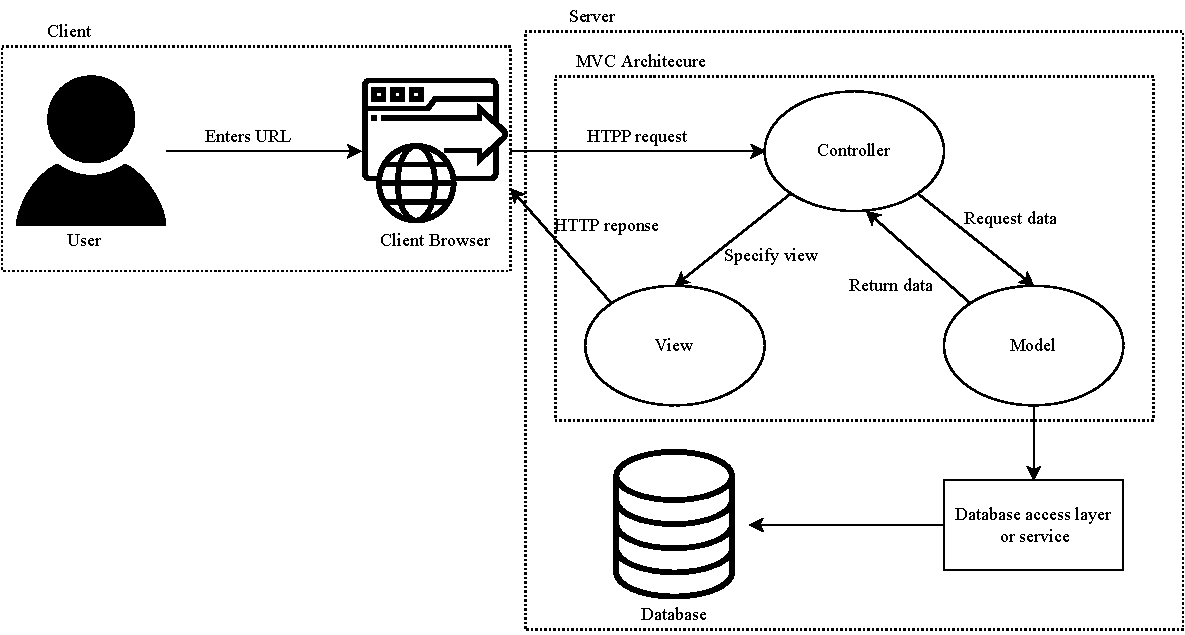
\includegraphics[width=0.9\textwidth]{Chapter2/Flow_MVC_Architecture/Flow_MVC_Architecture.pdf}
	\caption[MVC architecture for most web-based applications]
	{\textit{MVC architecture for most web-based applications \cite{Gu2010}}}\label{fig:ch2_flowMVC_Architecture}
\end{figure}

In \Cref{fig:ch2_flowMVC_Architecture} is the MVC architecture equivalent representation of \Cref{fig:ch2_systemDesign} where the data flow is shown of the MVC architecture. The user interacts with the Web application through their browser which will send a \textit{HTTP requests} to the \textit{Controller} and receive a \textit{HTTP response}\footnote{An \textbf{HTTP response} is made by a server to a client. The response aims to provide the client with the resource it requested, inform the client that the action it requested has been carried out; or else inform the client that an error occurred in processing its request. \cite{IBM2021a}.} from the \textit{View}.The \textit{Controller} will request and return the data to the \textit{Model} which interacts with the database access layer or service to do the \textit{create}, \textit{update} and \textit{delete} operations.\par To classify any interaction between the user (F/R 1) and server (F/R 2) to fulfil the functional requirements of \Cref{tbl:ch2_requirementsForUserActivtyEvent} only the \textit{HTTP request} are used for the logging points in \Cref{sec:ch2_loggingPoints} as it:

\begin{itemize}
	\item Meet the \ref{fr:requirementsUserBased1} and \ref{fr:requirementsUserBased1} as the user will interact with the \textit{View} to modify the data which needs to send back an \textit{HTTP request} to process the data on the \textit{Controller}.
	\item User activity types can be assigned for different scenarios that the user triggers when the request is being sent. 
	\item Any additional metadata can be sent with the \textit{request header}\footnote{A \textbf{request header} is an HTTP header that can be used in an HTTP request to provide information about the request context so that the server can tailor the response. For example, the Accept-$\ast$ headers indicate the allowed and preferred formats of the response. \cite{Mozilla2022}.} of the \textit{HTTP request}. This will reduce the overhead added by the logging mechanism by not sending additional \textit{HTTP request} each time back to the server when a user-based activity has been identified.
\end{itemize}

Most Web applications will make of use JavaScript to control the content of the page that is being displayed to the user. The primary method would be making use of an \textit{AJAX request} to communicate with the server to fulfil the user's action.\par The \textit{AJAX request} has some key features that will enable the logging points discussed in \Cref{sec:ch2_loggingPoints} to capture some logging attributes and classify the event as a user-based activity. \par The \texttt{beforeSend} setting of the \textit{AJAX request} enables tracking in real-time for the HTML element id and its HTML tag or other possible log attributes that need to be added to the request for the log point to capture it. The captured HTML element id, HTML tag and some other parameters can be added as a custom request header that will be sent to the server.

\begin{lstlisting}[caption={\textit{AJAX request example \cite{API.jQuery2022}}}, label={fig:ch2_ajaxBeforesend}]  
	$.ajax({
		url: "https://fiddle.jshell.net/favicon.png",
		beforeSend: function (xhr) {
			xhr.overrideMimeType("text/plain; charset=x-user-defined");
		}
	}).done(function (data) {
		if (console && console.log) {
			console.log("Sample of data:", data.slice(0, 100));
		}
	});
\end{lstlisting}

\subsection{Obtaining the element of user-based event}\label{sec:ch2_ElementObtaining}
In \Cref{sec:ch2_webApplicationArchitecture} the user-based activity event will be use a \textit{HTTP request} to send to the server when the user interacted with an \textit{HTML element}. For the functional requirements activity type (F/R 1.5.3) and metadata (F/R 1.5.6) in \Cref{tbl:ch2_keyLoggingAttributes} the \textit{HTML element} needs to be obtained to get the element's tag and identification text. This can be difficult to obtain due to \textit{bubbling}\footnote{\textbf{Bubbling} is when an event happens on an element, it first runs the handlers on it, then on its parent, then up on other ancestors. \cite{EventBubbling}.} that may occur when searching for the element that the user specifically interacted with.\par In \Cref{fig:ch2_event_bubbling} is the event propagation example of a child element that has been clicked on which executes a DOM event. The event propagation consists of three phases~\cite{EventBubbling}:

\begin{itemize}
	\item \textit{Capturing phase:} The event propagates downwards to the targeted element that the user interacted with.
	\item \textit{Target phase:} The event reaches the targeted element to execute the DOM event.
	\item \textit{Bubbling phase:} The event bubbles up from the targeted element
\end{itemize}

\begin{figure}[!htb] % An h :here, t: top, b: bottom.
	\centering % cent the figure
	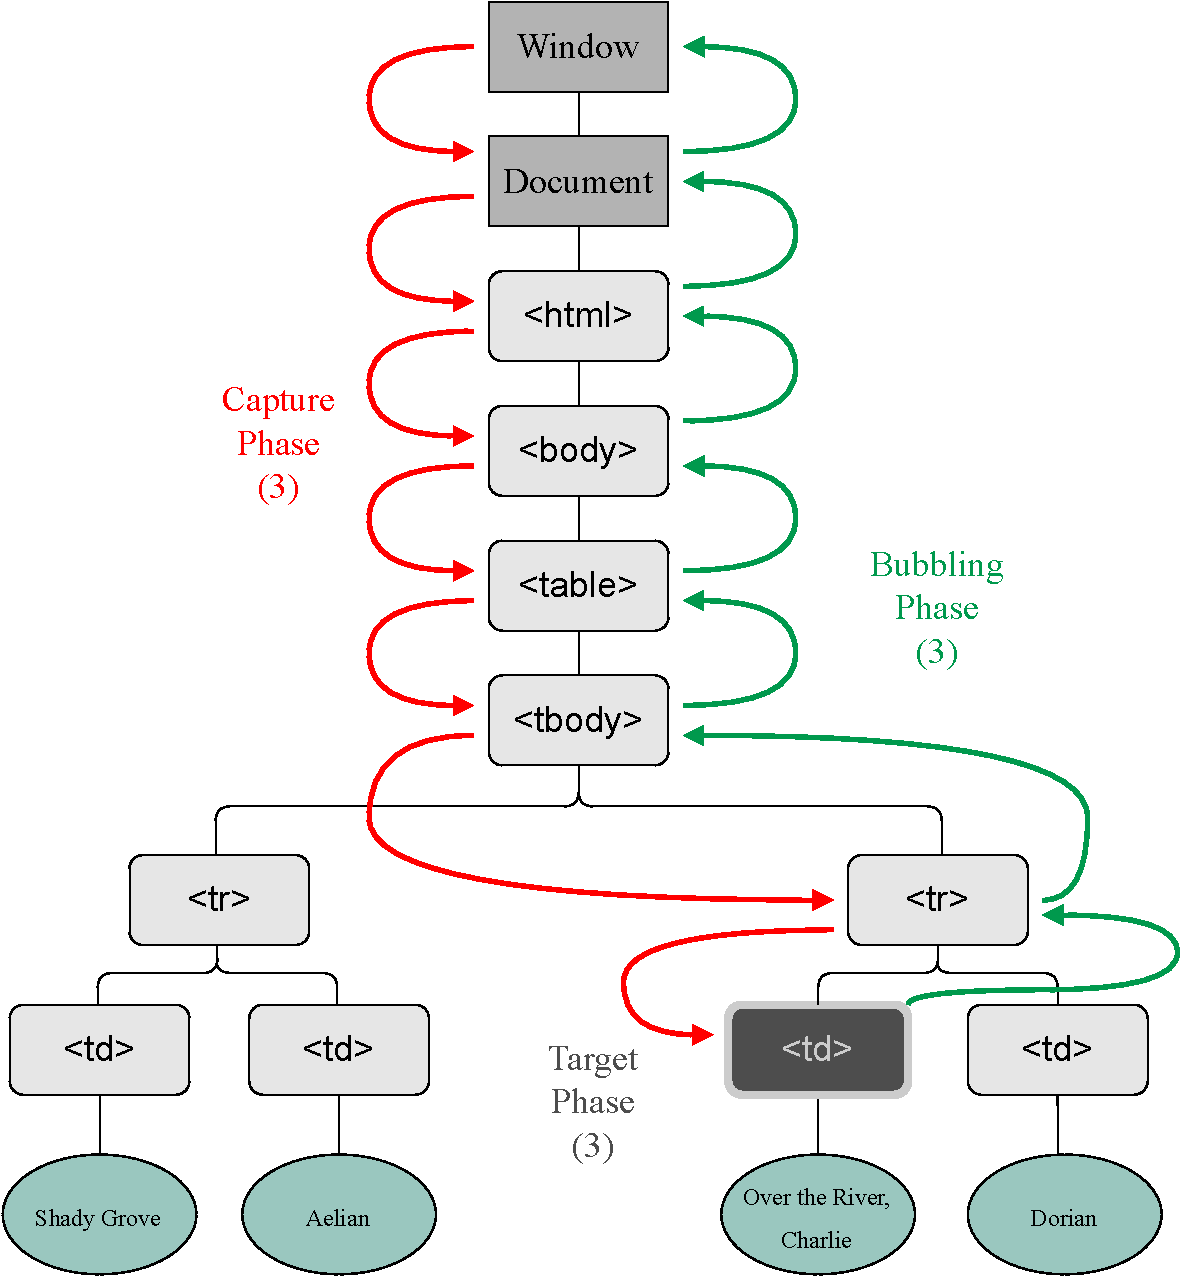
\includegraphics[width=0.6\textwidth]{Chapter2/event_bubbling/event_bubbling.pdf}
	\caption[JavaScript event propagation]
	{\textit{JavaScript event propagation~\cite{EventBubbling}}}\label{fig:ch2_event_bubbling}
\end{figure}

Capturing the targeted element may be difficult as some Web pages may have more complex HTML where the event propagation may sometimes not obtain the correct element information which the user interacted with. Another DOM event may have started during the initial element's event, therefore it is more accurate to obtain the targeted element by obtaining the last known element the user hovered over on the user interface.\par In \Cref{fig:ch2_element_event_capturing} is the flow diagram of to capture the element user interacted with for the user-based activity log. This code segment will be initiated during the \texttt{beforeSend} operation of the \textit{AJAX request} to filter HTML elements by a predefined allowed elements to use. Filtering the element tag names ensures that unwanted more complex elements or more basic elements that are not expected to be the initiator of the event will be used. \par If the Web location already changed or no element exists, the contents of the page might have already changed during the event propagation. The last known element that the user hovered on must be used as most likely might have been the element that the user interacted with. This will ensure there is always an element that has been detected and parsed with the request header in most UI changes.

\clearpage

\begin{figure}[!htb] % An h :here, t: top, b: bottom.
	\centering % cent the figure
	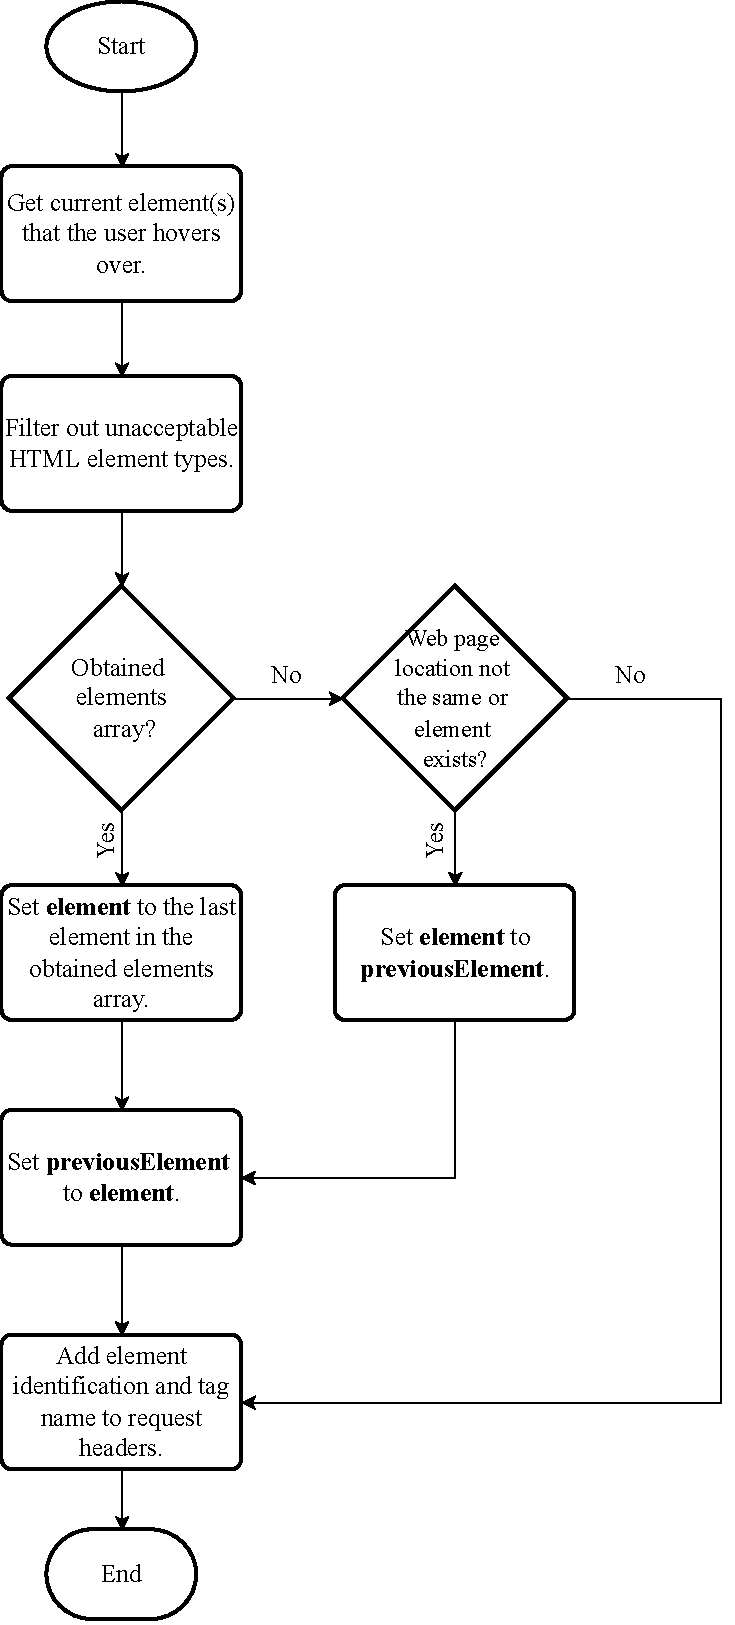
\includegraphics[width=0.5\textwidth]{Chapter2/element_capturing/element_capturing.pdf}
	\caption[HTML element capturing flow diagram]
	{\textit{HTML element capturing flow diagram}}\label{fig:ch2_element_event_capturing}
\end{figure}

\subsection{Client functional requirements interaction}
\par In \Cref{fig:ch2_user_based_actvity_classification} is the complete process of the user interacting with the UI to trigger a user-based activity event to be logged later for the client's functional requirements. It starts with the user interacting with the user interface. In the \texttt{beforeSend} operation of the \textit{AJAX request} the HTML element's id and tag should be attempted to. The default activity type is set to general activity (\ref{fr:uatType3}) until it is further processed later in the logging mechanism.\par If the activity has any additional metadata such as other request parameters, it will also be logged by adding searching for it in the \texttt{beforeSend} operation. The other metadata can also be captured in this stage from the client side like the element that the user clicked to initiate the event. The captured metadata is placed in a custom request header afterwards, and the \textit{AJAX request} continues its normal operations and sends the data back to the server.

\begin{figure}[!htb] % An h :here, t: top, b: bottom.
	\centering % cent the figure
	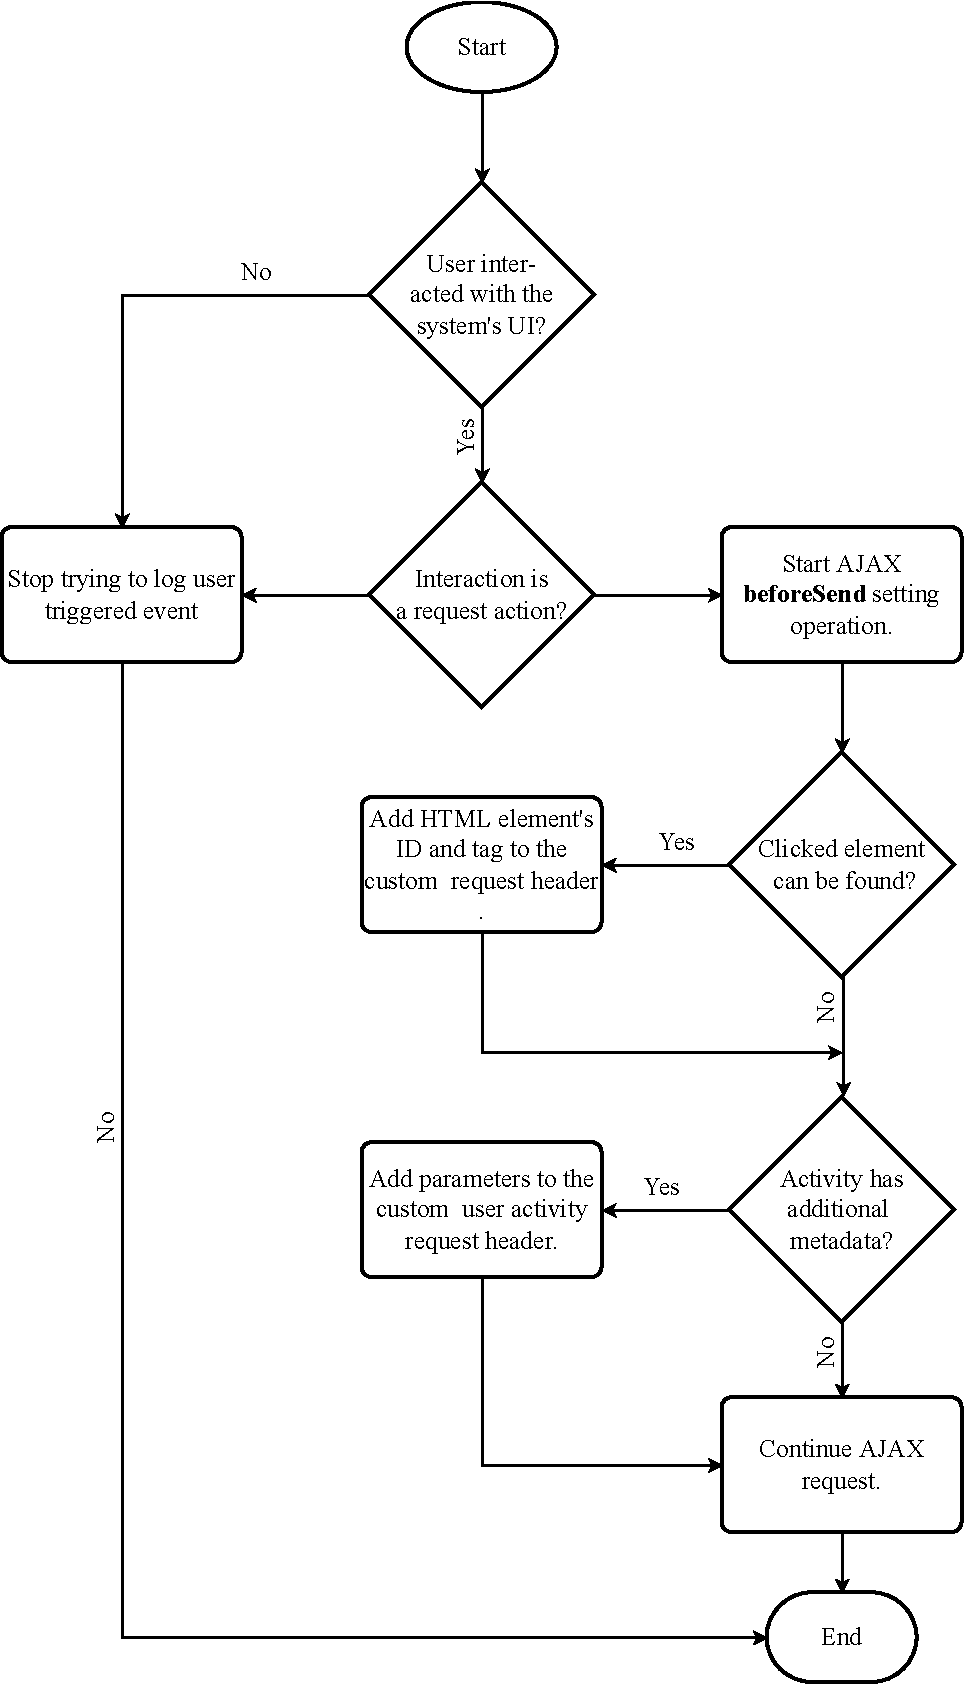
\includegraphics[width=0.75\textwidth]{Chapter2/client_functional_requirement_flow_diagram/client_functional_requirement_flow_diagram.pdf}
	\caption[User-based activity log classification flow diagram]
	{\textit{User-based activity log classification flow diagram}}\label{fig:ch2_user_based_actvity_classification}
\end{figure}

\clearpage

\subsection{Server side logging point}\label{sec:ch2_serverSideLoggingpoint}
In \Cref{sec:ch2_loggingPoints} the functional requirements for the logging point need to be fulfilled to create a suitable logging point for a software system to track user-based activities. The \textit{HTTP request} will call a function in the \textit{Controller} to execute the user's actions, these \textit{request} information can be obtained and parsed on to the logging point.\par The logging attribute can be created as a centralised code segment that all the software system's components can execute before executing the targeted software system in Web applications such as:

\begin{itemize}
	\item In frameworks like \texttt{C\#}'s \emph{.NET Framework}\footnote{\label{ftn:ch2_NetFramework}\textbf{.NET Framework} is a run-time execution environment that consists of common language run-time (\emph{CLR}) and a \texttt{.NET Framework Class Library} \cite{Harkness2007}.} the \textit{HTTP request} data can be extracted from the in build \textit{HTTP request} models to obtain the custom request headers set on the client side. Using the \texttt{ActionFilterAttribute} enables the creation of a global single logging point that can be called for every \textit{HTTP} function to execute the logging point first before continuing with the rest of the main targeted function. The rest of the log attributes can also be obtained during the execution of the filter by using the \texttt{FilterContext} to obtain:
	\begin{itemize}
		\item \textbf{Absolute URI path:} The string containing the absolute URI path of the currently active controller is part of the \texttt{FilterContext}. This does not reference the controller that handles the request at all times but the controller that the user is active on before initiating the request.
		\item \textbf{Absolute request URL:} The requested URL contains the targeted controller's name and function that the request needs to execute. 
		\item \textbf{Action parameters:} The \texttt{FilterContext} contains action parameters which are the request parameters sent with the AJAX request from the client device.
	\end{itemize}
	\item In other older Web applications that is created with programming languages such as \texttt{PHP} a more direct approach needs to be taken when accessing the request data. In this case, using multiple logging points that call the logging points' main code segment to capture the attributes and store the log in a database. The parameters may need to be extracted before parsing them to the main logging point code segment.
\end{itemize}

As long as the logging attributes and the \textit{HTTP request} headers are obtainable, the logging mechanism can be created on the server side to extract the data and process it. The activity type can be resolved by the defined cases e.g. if the request calls the \texttt{Index} function of the \textit{Controller} of the Web page, it can be identified as the Web page accessed user activity type (\ref{fr:uatType1}) of \Cref{tbl:ch2_userActivityTypes}.\par If the user-based event is using the \textit{Controller} or functions that modify the session, it can be classified as session changed event (\ref{fr:uatType3}) and the rest of the user-based activity events need to be tested afterwards if they meet certain criteria defined for the general activity types. If it fails all three types of classification the event is likely not user-generated or comes from \textit{AJAX request} that was executed after the initial first request. In such cases, the last HTML element id that triggered the event should not be listed as a clicked element in JavaScript.

\subsection{Storing the user-based actvity logs}\label{sec:ch2_databaseStorage}
In \Cref{sec:ch2_serverSideLoggingpoint} the logging point at the server side needs to extract the log attributes to be placed in the database. The database that is going to be used for the software system is a \texttt{MySQL} database.\par The captured parameters of the log attributes may have some sensitive user data that should not be logged. Functions can be excluded or assigned a new user activity type that will need to filter out certain parameters or not log any parameters a all. This will be any functions that include:

\begin{itemize}
	\item Session handling functions that contain passwords or other user information that should not be available for anyone but the user. This could lead to unintentional information disclosure of any personal information in the system utilisation analysis if it is available for anyone who can see and use the user-based activity logs,
	\item Complex parameters such as file upload streams of files that the user tries to upload. This information cannot be broken down to a simple \texttt{JSON} structure as in \Cref{fig:ch2_MetadataJsonExample}, other metadata such as the file size, name and type can rather be logged. This can also be defined as a separate user-based activity event type by detecting these complex parameters.
\end{itemize}

In \Cref{tbl:ch2_SQLLoggingTable} is the SQL data type of the parameters and the functional requirements that it needs will need to fulfill of \Cref{tbl:ch2_keyLoggingAttributes}. Additional for more modern systems such as the \texttt{C\#}'s \textit{.NET Framework} the request origin (\ref{fr:lpa5}) can be split into two different fields:

\begin{itemize}
	\item The \textbf{Area} is the subsystems where different MVC systems are grouped. 
	\item The \textbf{Controller} this field will only contain the name of the controller that executes the request. 
\end{itemize}

\begin{table}[!htb]
	\centering
	\caption[Log attributes for SQL table]
	{\textit{Log attributes for SQL table}}
	\label{tbl:ch2_SQLLoggingTable}
	\begin{tabularx}{\textwidth}{|X|X|X|}
		\hline \textbf{Column Name} & \textbf{SQL Data Type} & \textbf{Requirement} \\
		\hline \textbf{ActivityID} & INT(11) & \ref{fr:lpa1} \\
		\hline \textbf{Timestamp} & DATETIME & \ref{fr:lpa2} \\
		\hline \textbf{ActivityType} & ENUM & \ref{fr:lpa3} \\
		\hline \textbf{UserID} & INT(4) & \ref{fr:lpa4} \\
		\hline \textbf{Subsystem} & VARCHAR(45) & \ref{fr:lpa5} \\
		\hline \textbf{Controller} & TEXT & \ref{fr:lpa5} \\
		\hline \textbf{GroupID} & INT(4) & \ref{fr:lpa7} \\
		\hline \textbf{MetaData} & JSON & \ref{fr:lpa6} \\
		\hline
	\end{tabularx}
\end{table}

The log attributes in \Cref{tbl:ch2_SQLLoggingTable} will have foreign key references to other tables in the database. In \Cref{fig:ch2_erdOfEventLogs} is an ERD diagram that describes the relationship of the table created to store the log attributes with other relevant tables. In the system utilisation analysis, this enables different fields of the other tables to be used to categorise the logs.

\clearpage

\begin{figure}[!htb] % An h :here, t: top, b: bottom.
	\centering % cent the figure
	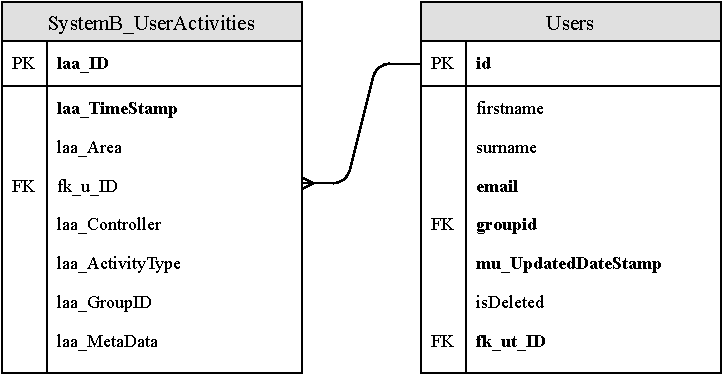
\includegraphics[width=0.99\textwidth]{Chapter2/SystemB_ERD_Basic/SystemB_ERD_Basic.pdf}
	\caption[ERD of user activities]
	{\textit{ERD of the user activities}}\label{fig:ch2_erdOfEventLogs}
\end{figure}

\subsection{Server side log parsing}
In \Cref{fig:ch2_loggingParse} is the server side log parsing of the obtained possible user-based activity events using for a \emph{.NET Framework} software system. The defined \texttt{ActionFilterAttribute} will start the user-based activity process before the targeted process is executed. At this stage, if anything goes wrong with the logging at during the execution of this filter, it should be abandoned and let the software system continue to ensure that it doesn't interfere with the software system's operations (\ref{fr:lpa4} of \Cref{tbl:ch2_loggingPointRequirement}).\par In the case of the request method \texttt{NULL} or empty due to errors such as incorrect parameter types for the targeted procedure in the controller, the logging point should stop attempting to log the user-based log. The issue would most likely appear as a runtime error and any user-based activity logging procedures will also fail due to incomplete data or cause the logs to be not complete and consistent (\ref{fr:lpa3} of \Cref{tbl:ch2_loggingPointRequirement}).\par If the captured user-activity log contains any parameters it should be checked for any session-related parameters or any other potential user data that should be removed from the metadata to prevent any personal information from being accessed by not the owner of the user account. If it doesn't contain any request parameters the \texttt{ElementInfo} should be set to \texttt{NULL}.\par The \texttt{ElementInfo} contains all the metadata send from the client side logging point that captured the HTML element data in \Cref{fig:ch2_element_event_capturing}. In \Cref{fig:Ch2_ElementInfo} is the \texttt{JSON} data of the \texttt{ElementInfo} which consist of:

\begin{itemize}
	\item \texttt{ElementTagName}, is the HTML element's tag name which is one of the defined accepted tag names such as \texttt{button}, \texttt{label} and \texttt{td} etc.,
	\item \texttt{ElementID}, identification of the element if it has been assigned to the element and can be obtained on the client side,
	\item \texttt{ElementDataKey}, additional captured data attributes that expands on the elements identity if it is a custom made HTML element control. Some software systems may have other custom-created HTML elements which also can trigger a user-based activity. It can be other miscellaneous elements such as a \texttt{label} which are not normal input controls.
\end{itemize}

\clearpage

\begin{lstlisting}[style=json, caption={\textit{Element properties JSON}}, label={fig:Ch2_ElementInfo}] 
	{ "ElementTagName" : "button",
		"ElementID" : "submitButton",
		"ElementDataKey": "submit-control"		
	}
\end{lstlisting}

If the \texttt{FilterContext}'s requested procedure is called and it is the \texttt{Index} which is the first procedure that needs to be executed for a Web page being accessed. This activity type is the first user activity type at this point of the log parsing before it is processed again to another user activity type. \par If it is not the \texttt{Index} the process will continue to the next operation which check's if the \texttt{ElementInfo}'s \texttt{ElementDataKey} is either a null or empty value. If there is any data available the activity type can be set to the custom control defined activity type or just custom control to represent all these custom-made elements. The \texttt{ElementID} is set to custom control element or the defined custom control's identification. \par If the \texttt{ElementInfo}'s \texttt{ElementDataKey} is null or a empty value the user activity type is set to the element's defined activity type. After the activity type is resolved the request origin of the user-based activity is obtained by getting the request's absolute path.\par After the request origin has been obtained, other relevant session information such as the group that represents a certain entity data can be obtained as well as the user's identification and other relevant metadata that is available at this stage to complete the log attributes that needs to captured from \Cref{tbl:ch2_keyLoggingAttributes} to complete the user-based activity log.\par The data is parsed to the activity logger that will write the log into a database if the log was successfully obtained. This will end the logging process until a new user-based event log is ready to be processed and stored in the database.

\begin{figure}[!htb]
	\centering
	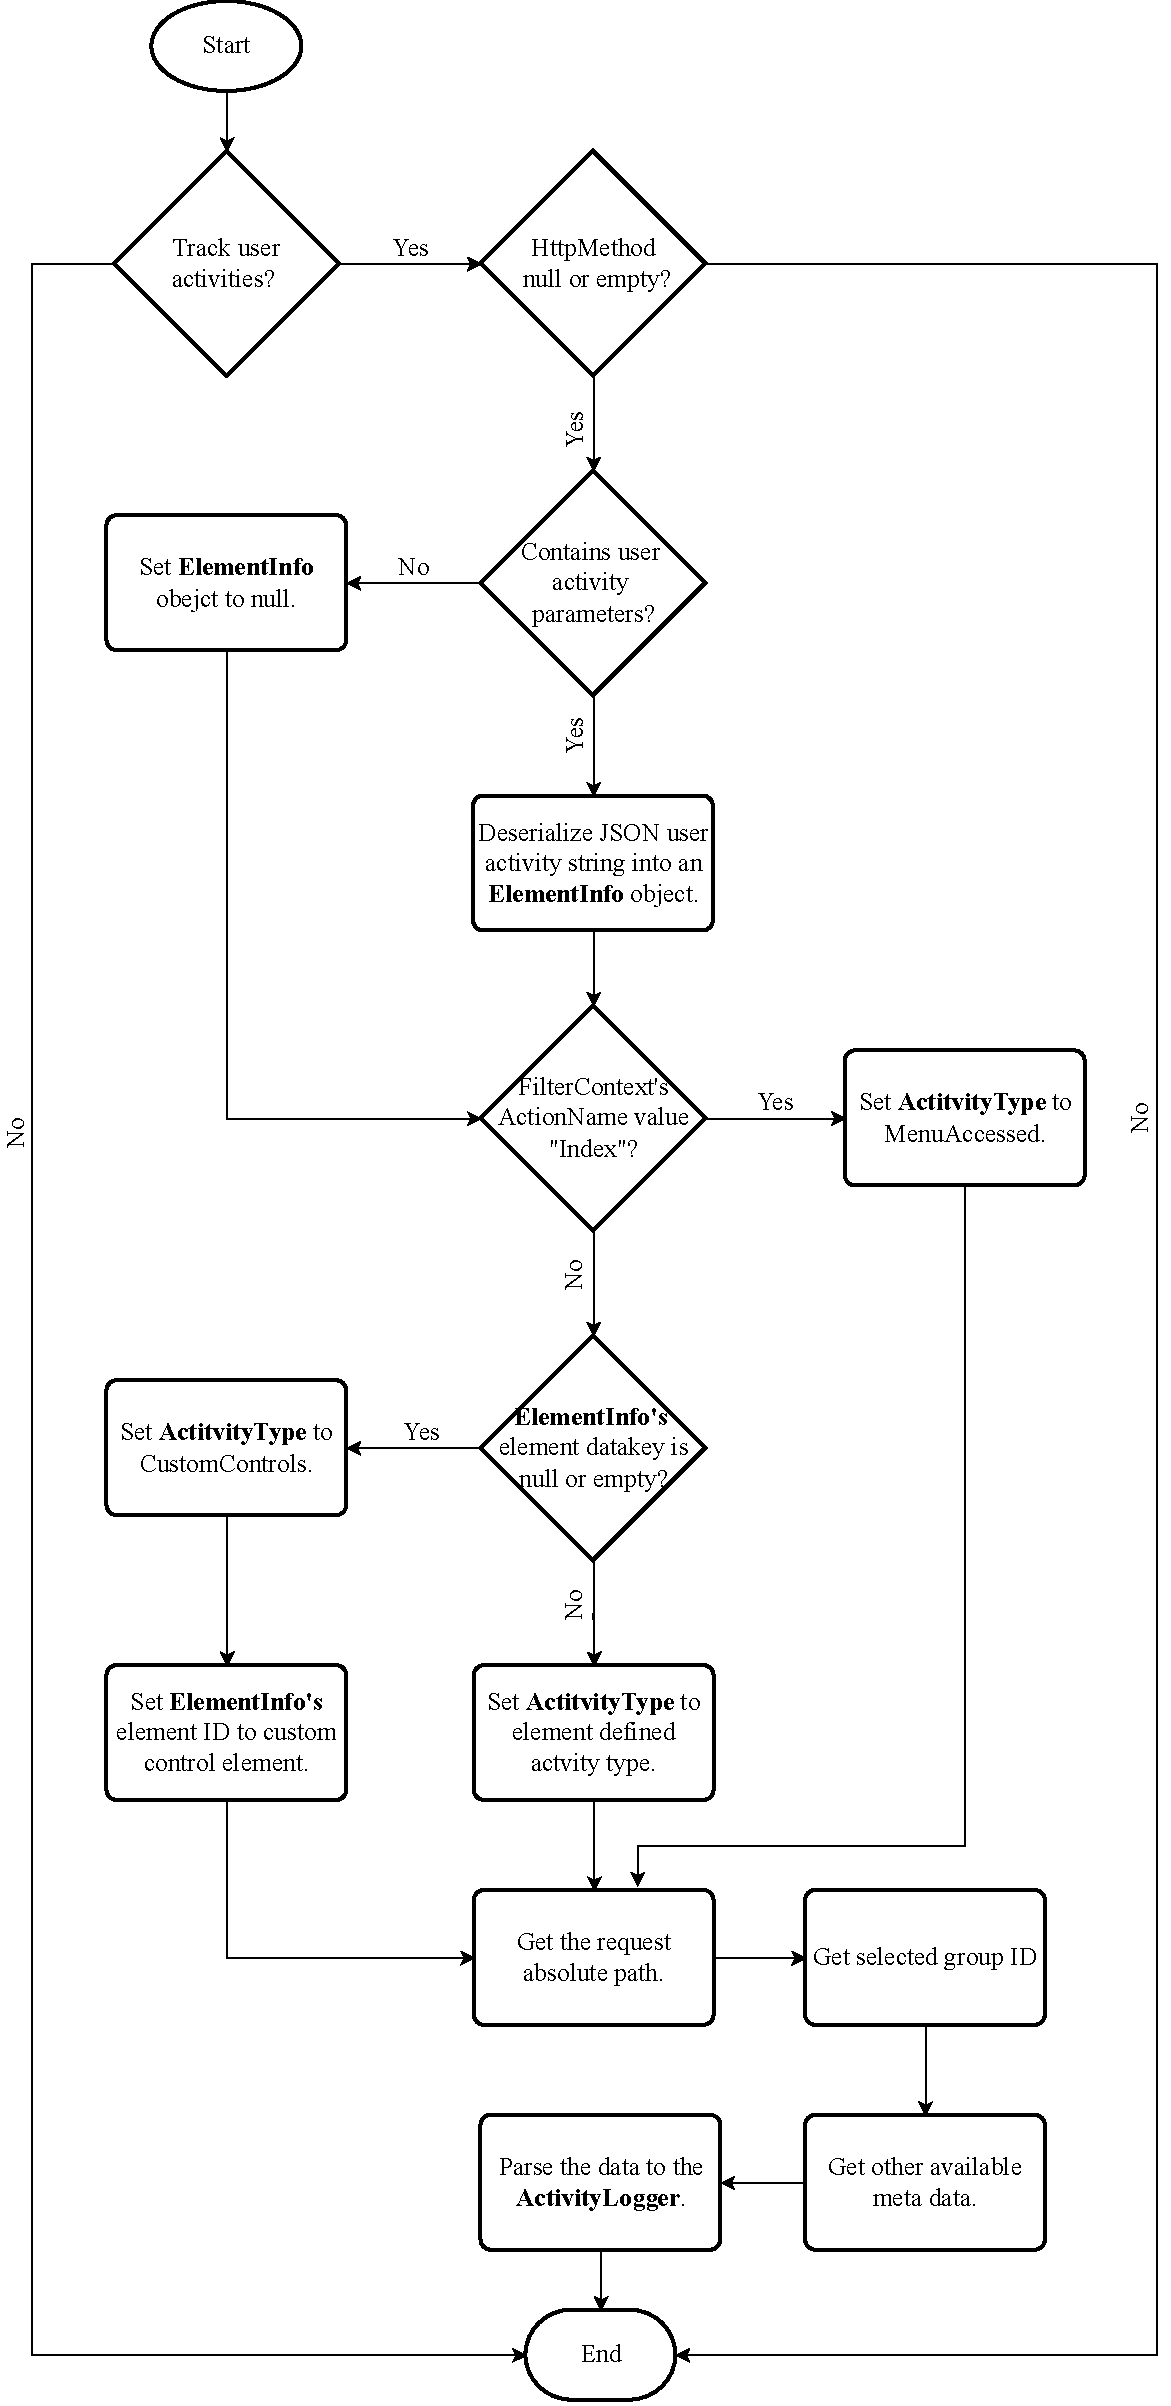
\includegraphics[width=0.7\textwidth]{Chapter2/SystemB_FilterContext/SystemB_FilterContext.pdf}
	\caption[Server side log parsing flow diagram]
	{\textit{Server side log parsing flow diagram}}\label{fig:ch2_loggingParse}
\end{figure}

\clearpage

\section{System utilisation analysis}\label{ch2:sec_system_utilisation_analysis}
The system utilisation analysis will make use of a Web-based graphical user interface to view the raw logs stored in the database and use any other visualisation tools for data insights of the user-based activities. In \Cref{tbl:ch2_utilisation_requirements} is the functional requirements for the utilisation analysis.

\setcounter{phase}{3}
\setcounter{subphase}{0}
\begin{table}[!htb]
	\centering
	\caption[System utilisation analysis functional requirements]
	{\textit{System utilisation analysis functional requirements}}
	\label{tbl:ch2_utilisation_requirements}
	\begin{tabularx}{\textwidth}{|l|l|X|}
		\hline \textbf{Requirement ID} & \textbf{Requirement name} & \textbf{Description} \\
		\hline \subphase{fr:ur1} & Log availability & \RaggedRight The user-based logs should be available for any defined period the logging mechanism was actively capturing the user-based events. \\
		\hline \subphase{fr:ur2} & Log completeness & \RaggedRight The user-based logs should be complete and there should be minimal corrections made post logging during the log extraction process (\ref{fr:ur3}) and visualization presentation (\ref{fr:ur4}). \\
		\hline \subphase{fr:ur3} & Log extraction & \RaggedRight The user-based logs are extracted from the database and imported into a visualization presentation (\ref{fr:ur4}) for the user-based activity logs. \\
		\hline \subphase{fr:ur4} & Log visual presentation & The visual presentation of the extracted logs should be shown to the user that will make use of the activity logs in a custom visual system or make use of other third-party tools. This will impact how the logs will be extracted (\ref{fr:ur4}) from the database as third-party systems may make use of an API to get the logs from the database. \\
		\hline \subphase{fr:ur5} & Log comparison & \RaggedRight By Using the F/R 3.2 the utilisation between different log attributes that are used as the defined criteria. This will be to group and compare different types of users, subsystems and activity types against each other etc.\\
		\hline \subphase{fr:ur6} & \RaggedRight Maintenance suggestion & Maintenance suggestions can be made from the system utilisation reports by prioritising maintenance or decommissioning software systems. This can be data or visual representations of the log comparison (\ref{fr:ur5}) using the log visual presentation systems (\ref{fr:ur6}) or creating a summary report from the visual presentation that contains the maintenance suggestions. \\
		\hline
	\end{tabularx}
\end{table}

\clearpage

Each of these functional requirements ensures that the system utilisation analysis will be achieved for the created logging mechanism in \Cref{Ch2:LoggingMechanism}. The main user interface of the system utilisation analysis will consist of the presentation of the user-based activities (\ref{fr:ur4}). This system will either be a custom-created system to display these log or third-party software such as Microsoft's business intelligence platform, PowerBI. \par Using the third-party tools has advantages over creating custom software for the visual presentation (\ref{fr:ur4}):

\begin{itemize}
	\item Thrid-party business intelligence platforms have all the necessary analytical functionality. The tables and charts needed for the visual presentation can be created with minimal programming difficulty.
	\item The advanced tools in these third-party business intelligence platforms provide more ways the user-based activity logs can be visualised for the log comparison (\ref{fr:ur5}).
	\item Maintenance and editing of these third-party representations are mostly trouble-free to do. The amount of support and guides that should be available to the developer instead of relying on the creator or other developers that are available to make updates to the custom visual presentation.
\end{itemize}

These third-party tools do indeed have some other drawbacks such as:

\begin{itemize}
	\item Third-party business intelligence platforms most likely will require some sort of subscription that can be very costly for a company licence.
	\item Extra courses might be needed to fully use the capabilities of these platforms.
	\item Additional functionality such as APIs might be needed for the log extraction (\ref{fr:ur3}) to import the data to the platform.
\end{itemize}

With the drawbacks listed above the third-party business intelligence platforms is the better visual presentation tools for the system utilisation analysis if it is available for use than creating and managing a custom visualisation platform.

\subsection{Log availability and completeness}\label{sec:ch2_log_Availability}
The log availability (F/R 3.1) and completeness (F/R 3.2) functional requirements can be achieved all the functional requirements of the user-based activity log in \Cref{sec:ch2_requirementsOfUAT} are accomplished with minimal processing of the raw logs afterwards. There will be always changes made to the system that can impact which possible user-based events are considered to be logged.

\subsection{Log extraction and visual presentation}\label{sec:ch2_logExtraction}
Log extraction refers to the methods used to obtain the logs from the database with any other relevant data that can be used in the visualisation presentation (\ref{fr:ur4}). The raw logs will need to make use of the foreign references to other tables in the database to provide more detail about the user-based event log as in \Cref{fig:ch2_erdOfEventLogs}.\par In \Cref{fig:ch2_pbiExample} is an example of a visual presentation of Microsoft's PowerBI report that displays imported data. These reports will contain the extracted data of \Cref{fig:ch2_erdOfEventLogs} using either an API or will extract the data like the rest of the system if it is a custom visualisation.

\begin{figure}[!htb] % An h :here, t: top, b: bottom.
	\centering % cent the figure
	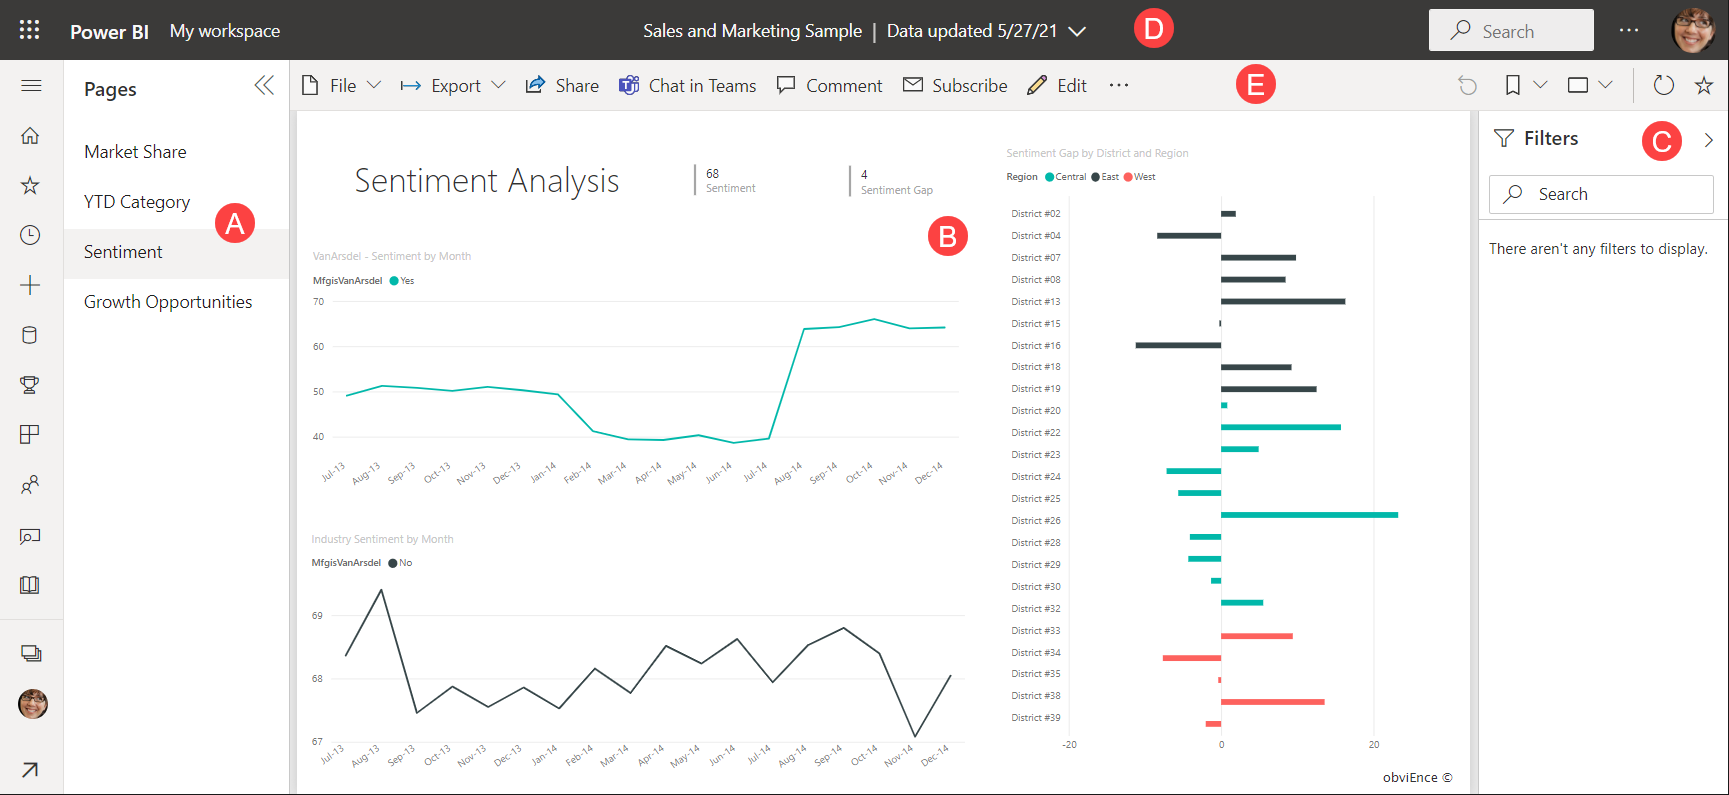
\includegraphics[width=0.75\textwidth]{Chapter2/normal_images/power_bi_report.png}
	\caption[Example of a visual presentation]
	{\textit{Example of a visual presentation}}\label{fig:ch2_pbiExample}
\end{figure}

\subsection{Maintenance improvements}\label{sec:ch2_utilisationImprovements}
The system utilisation analysis aims to provide maintenance recommendations to the developers to improve their maintenance efforts by:

\begin{itemize}
	\item Prioritising the maintenance efforts on more frequently used systems.
	\item Decommission unused systems. The user-based activities provide a quantitative reason why certain systems can be decommissioned due to inactivity from the users.
\end{itemize}

\begin{table}[!htb]
	\centering
	\caption[System utilisation analysis categories]
	{\textit{System utilisation analysis categories}}
	\label{tbl:ch2_utilisationCategories}
	\begin{xltabular}{\textwidth}{|l|l|X|}
		\hline \textbf{Requirement ID} & \textbf{Requirement name} & \textbf{Description} \\
		\hline \subsubphase{fr:utCategories1} & Users & The users of the software systems can be put in different categories based on who uses the software. This can be both the customer users or the employees using the software. Using the activities of the customer users will provide the data on which systems the development team needs to put their resources into. \\
		\hline \subsubphase{fr:utCategories2} & User activity types & The user activity types in \Cref{tbl:ch2_userActivityTypes} can be used as a category to compare different user-based activity types with each other and use a sub-category for categories such as the different users that can use the system (\ref{fr:utCategories1}). \\
		\hline \subsubphase{fr:utCategories3} & Subsystem or controllers & The request origin (\ref{fr:lpa5}) of the user-based activities can be categorise to compare different subsystems and controllers to each other.\\
		\hline \subsubphase{fr:utCategories3} & Miscellaneous categories & This user-based activity category type will make use of the metadata attribute (\ref{fr:lpa7}) of \Cref{tbl:ch2_keyLoggingAttributes}. The other fields which are not set as main categories can be also placed in this category as they can take multiple forms.\\
		\hline
	\end{xltabular}
\end{table}

\clearpage

\section{Verification}\label{sec:ch2_verification}
Using the functional requirements definded in \Cref{Ch2:LoggingMechanism,ch2:sec_system_utilisation_analysis} the system can be verified that it satisfies the system requirements in \Cref{tbl:ch2_verification}.

\begin{table}[!htb]
	\centering
	\caption[System requirements for verification]
	{\textit{System requirements for verification}}
	\label{tbl:ch2_verification}
	\begin{tabularx}{\textwidth}{|X|l|c|}
		\hline \textbf{Requirement} & \textbf{Methodology reference} & \textbf{Requirement met} \\
		\hline \textbf{User activity types} & \Cref{sec:ch2_requirementsOfUAT,sec:ch2_userActivityTypes} & \Checkmark \\
		\hline \textbf{Log attributes} & \Cref{sec:ch2_logAttributes} & \Checkmark \\
		\hline \textbf{Logging points} & \Cref{sec:ch2_loggingPoints,sec:ch2_webApplicationArchitecture,sec:ch2_ElementObtaining,sec:ch2_serverSideLoggingpoint} & \Checkmark \\
		\hline \textbf{Log extraction and visualisation} & \Cref{sec:ch2_databaseStorage,sec:ch2_logExtraction} & \Checkmark \\
		\hline \textbf{System utilisation analysis} & \Cref{sec:ch2_utilisationImprovements} & \Checkmark \\
		\hline
	\end{tabularx}
\end{table}

\section{Conclusion}
In \Cref{Ch2:LoggingMechanism} are the defined functional requirements for a logging mechanism for the system utilisation analysis in \Cref{ch2:sec_system_utilisation_analysis}. The user activity types defined in \Cref{sec:ch2_userActivityTypes} are the base of what log attributes need to be logged to create a user-based log.\par The logging points captured logs and send them to the server's logging point where it is processed and stored in writing to a database.\par The logs are extracted into a visual presentation which enables the maintenance improvement suggestions based on the utilization analysis in \Cref{ch2:sec_system_utilisation_analysis}.